\chapter{Neural Networks}

\section{Biological Inspiration}

Artificial neural networks were inspired by the human brain, one of the most efficient information-processing systems found in nature. Although artificial neural networks are much simpler than biological brains, they were developed by adopting the basic principle of how biological neurons receive, process, and transmit information.

A biological neuron consists of three main components. The \textbf{dendrites} receive electrical signals from other neurons, the \textbf{cell body} (or soma) integrates these incoming signals, and the \textbf{axon} transmits the resulting signal to other neurons through specialized connections called synapses. A neuron generates an electrical impulse only when the combined incoming signals exceed a certain threshold, allowing information to propagate throughout the nervous system.

\begin{figure}[h]
    \centering
    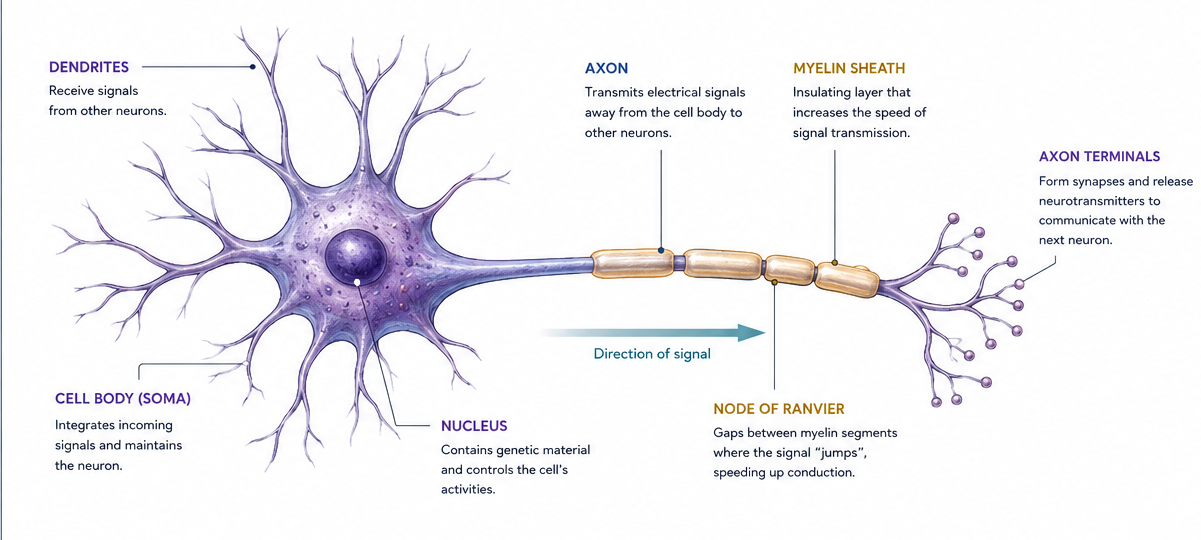
\includegraphics[width=0.95\textwidth]{figures/1-0.png}
\end{figure}
Inspired by this mechanism, Warren McCulloch and Walter Pitts proposed the first mathematical model of an artificial neuron in 1943. Although highly simplified, their model demonstrated that a neuron could be represented as a computational unit capable of receiving multiple inputs, combining them, and producing an output. This work laid the foundation for the development of artificial neural networks.

It is important to note that artificial neurons are not intended to accurately replicate the biological brain. Instead, they capture only its essential computational principle: combining multiple inputs to produce an output. This simple idea forms the basis of all modern neural network architectures.


\section{Artificial Neural Networks}

Artificial Neural Networks (ANNs) are computational models composed of interconnected processing units called \textbf{artificial neurons}. Inspired by the structure of the human brain, these networks are designed to learn relationships between input data and desired outputs by adjusting their internal parameters during training.

An artificial neural network is organized into layers of neurons through which information flows sequentially. Each neuron receives information from neurons in the previous layer, performs a simple mathematical computation, and passes its output to the next layer. By combining the outputs of many interconnected neurons, the network is capable of solving increasingly complex problems.

A typical feedforward neural network consists of three types of layers:

\begin{itemize}
    \item \textbf{Input Layer:} Receives the input features from the dataset.
    \item \textbf{Hidden Layer(s):} Process the information and extract increasingly meaningful representations.
    \item \textbf{Output Layer:} Produces the final prediction of the network.
\end{itemize}

The basic computational unit of the network is the artificial neuron. Each neuron receives one or more input values, combines them using trainable parameters called \textbf{weights}, adds a \textbf{bias} term, and computes

\begin{equation}
z=\sum_{i=1}^{n}w_i x_i+b.
\end{equation}

The computed value is then passed through an \textbf{activation function}, which determines the neuron's output. By connecting many neurons together, the network can gradually transform raw input data into increasingly useful representations.

During training, the network automatically adjusts its weights and biases to minimize prediction errors. As a result, the network gradually learns the relationship between the input data and the desired output.

The simplest neural network consists of a single artificial neuron and is known as the \textbf{Perceptron}. Although simple, the Perceptron introduced the fundamental principles upon which modern deep learning models are built.
\section{Perceptron}

The \textbf{Perceptron} is the simplest form of an artificial neural network and the first computational model capable of learning from data. Proposed by Frank Rosenblatt in 1958, it extended the earlier McCulloch--Pitts neuron by introducing a learning mechanism that automatically adjusts its parameters using training examples. This innovation marked an important milestone in the development of machine learning and laid the foundation for modern neural networks.

A Perceptron consists of a single artificial neuron that receives one or more input values and produces a binary output. Like every artificial neuron, it combines the inputs using trainable weights, adds a bias term, and computes a weighted sum given by

\begin{equation}
z=\sum_{i=1}^{n}w_i x_i+b.
\end{equation}

The weighted sum is then passed through a \textbf{threshold activation function}, also known as the step function, which determines the final output:
\clearpage
\begin{equation}
\hat{y}=
\begin{cases}
1, & z \geq 0,\\
0, & z < 0.
\end{cases}
\end{equation}

\begin{figure}[h]
    \centering
    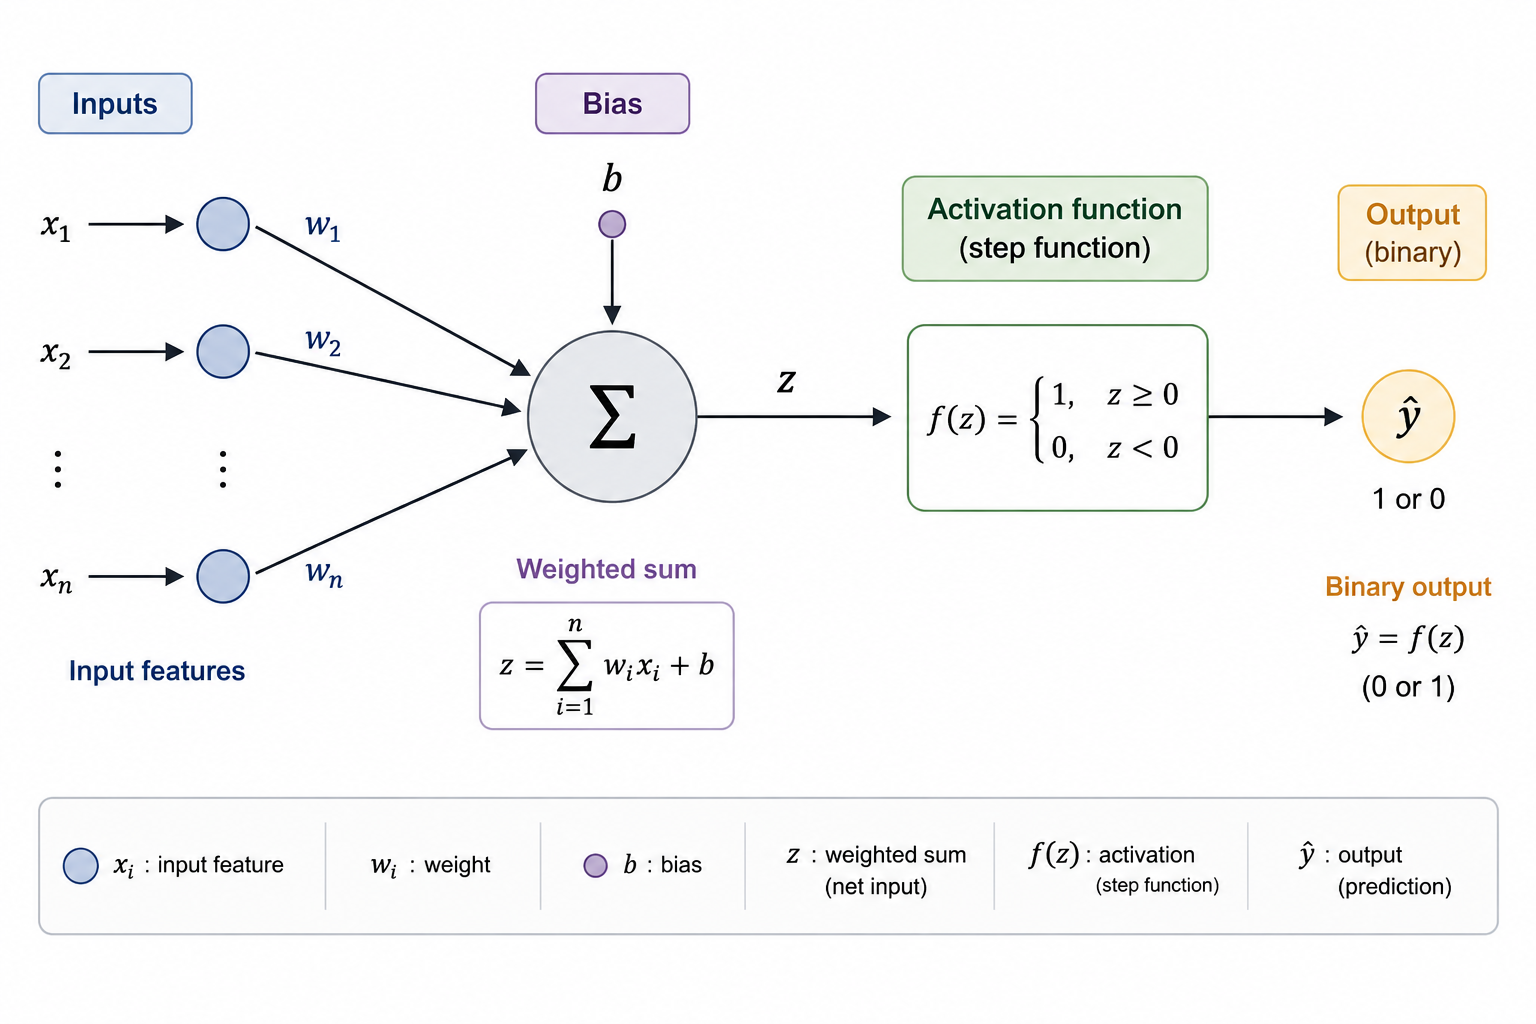
\includegraphics[width=0.95\textwidth]{figures/1-1.png}
\end{figure}

The Perceptron is therefore a \textbf{binary classifier}, meaning that it can assign an input to one of two possible classes. Geometrically, it does so by learning a \textbf{linear decision boundary} that separates the classes. In two-dimensional space, this boundary is represented by a straight line; in higher dimensions, it is referred to as a hyperplane.
\begin{figure}[h]
    \centering
    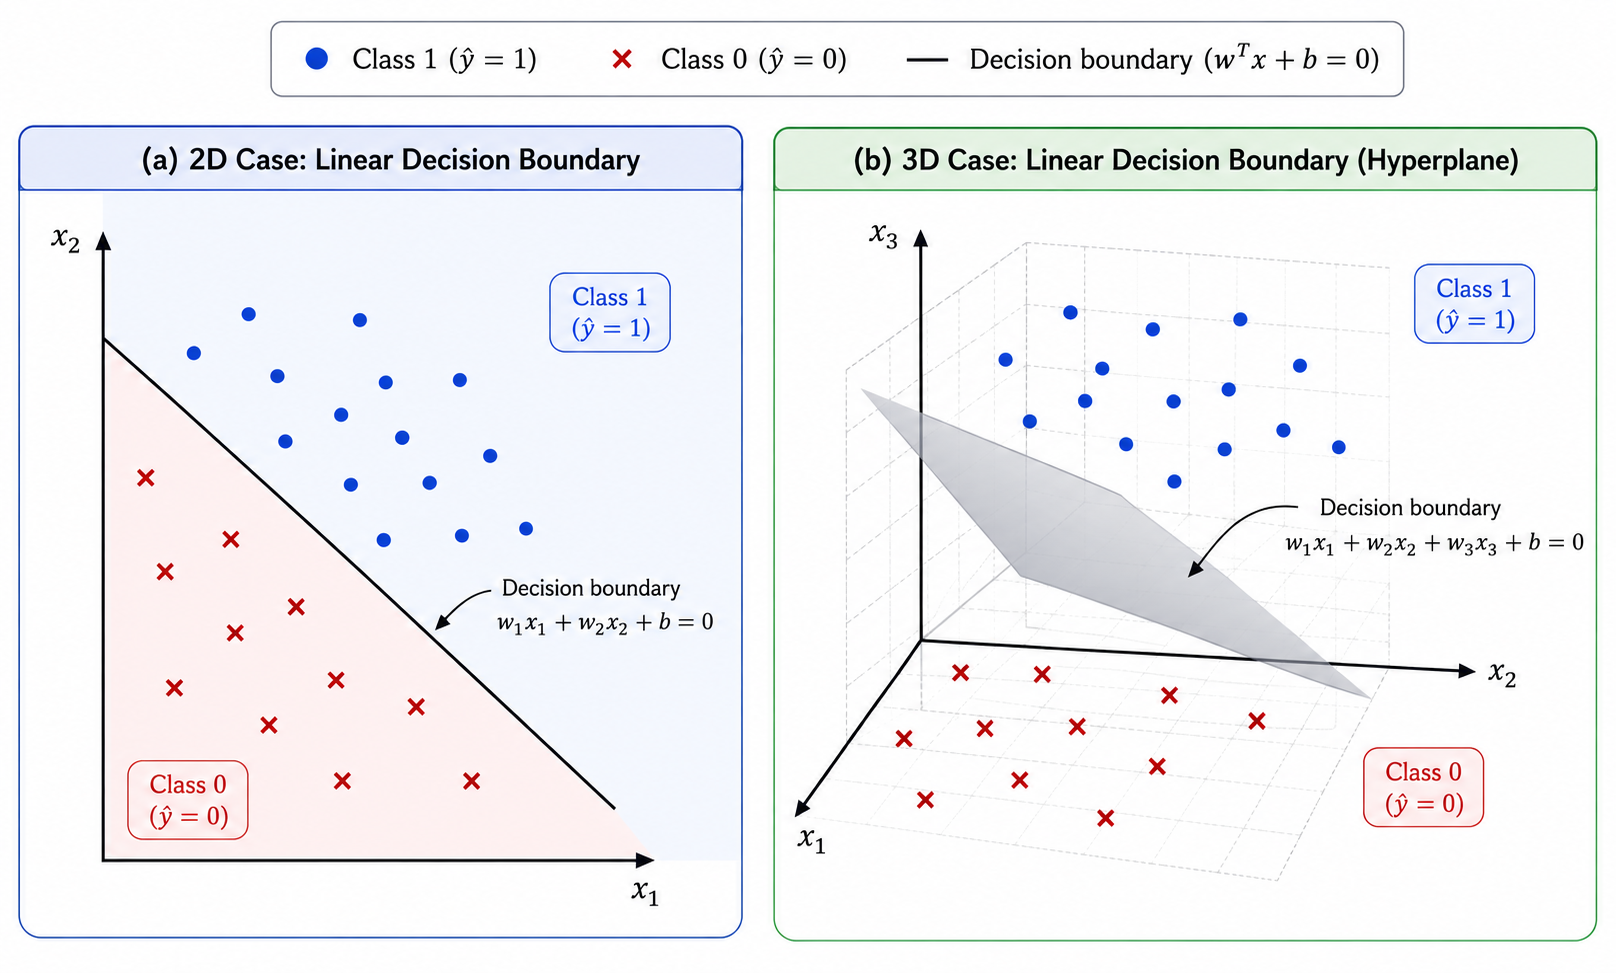
\includegraphics[width=0.95\textwidth]{figures/first.png}
\end{figure}
Despite its simplicity, the Perceptron introduced several fundamental concepts that remain at the core of modern deep learning, including trainable parameters, prediction, and learning from data. 
\section{Perceptron Learning Algorithm}

The distinguishing feature of the Perceptron is its ability to learn automatically from data. Rather than manually selecting the values of the weights and bias, the Perceptron adjusts these parameters during training so that its predictions become increasingly accurate. This process is known as the \textbf{Perceptron Learning Algorithm}.

The algorithm begins by initializing the weights and bias, typically with small random values or zeros. The training dataset is then presented to the model one example at a time. For each training sample, the Perceptron computes the weighted sum, applies the threshold activation function, and produces a predicted output.

The prediction is compared with the true class label to determine whether the classification is correct. If the prediction is correct, no changes are made to the model parameters. Otherwise, the weights and bias are updated according to the Perceptron learning rule.

Let $y$ denote the true class label and $\hat{y}$ the predicted output. The prediction error is defined as

\begin{equation}
e = y - \hat{y}.
\end{equation}

The weights are updated using

\begin{equation}
w_i \leftarrow w_i + \eta e x_i,
\end{equation}

while the bias is updated as

\begin{equation}
b \leftarrow b + \eta e,
\end{equation}

where $\eta$ is the \textbf{learning rate}, a positive constant that controls the magnitude of each update.

This procedure is repeated for all training samples. After one complete pass through the dataset, called an \textbf{epoch}, the algorithm starts another pass using the updated parameters. Training continues until the Perceptron correctly classifies all training examples or until a predefined number of epochs is reached.
\vspace{3cm}
The complete learning procedure can be summarized as follows:
\clearpage
\begin{figure}[h]
    \centering
    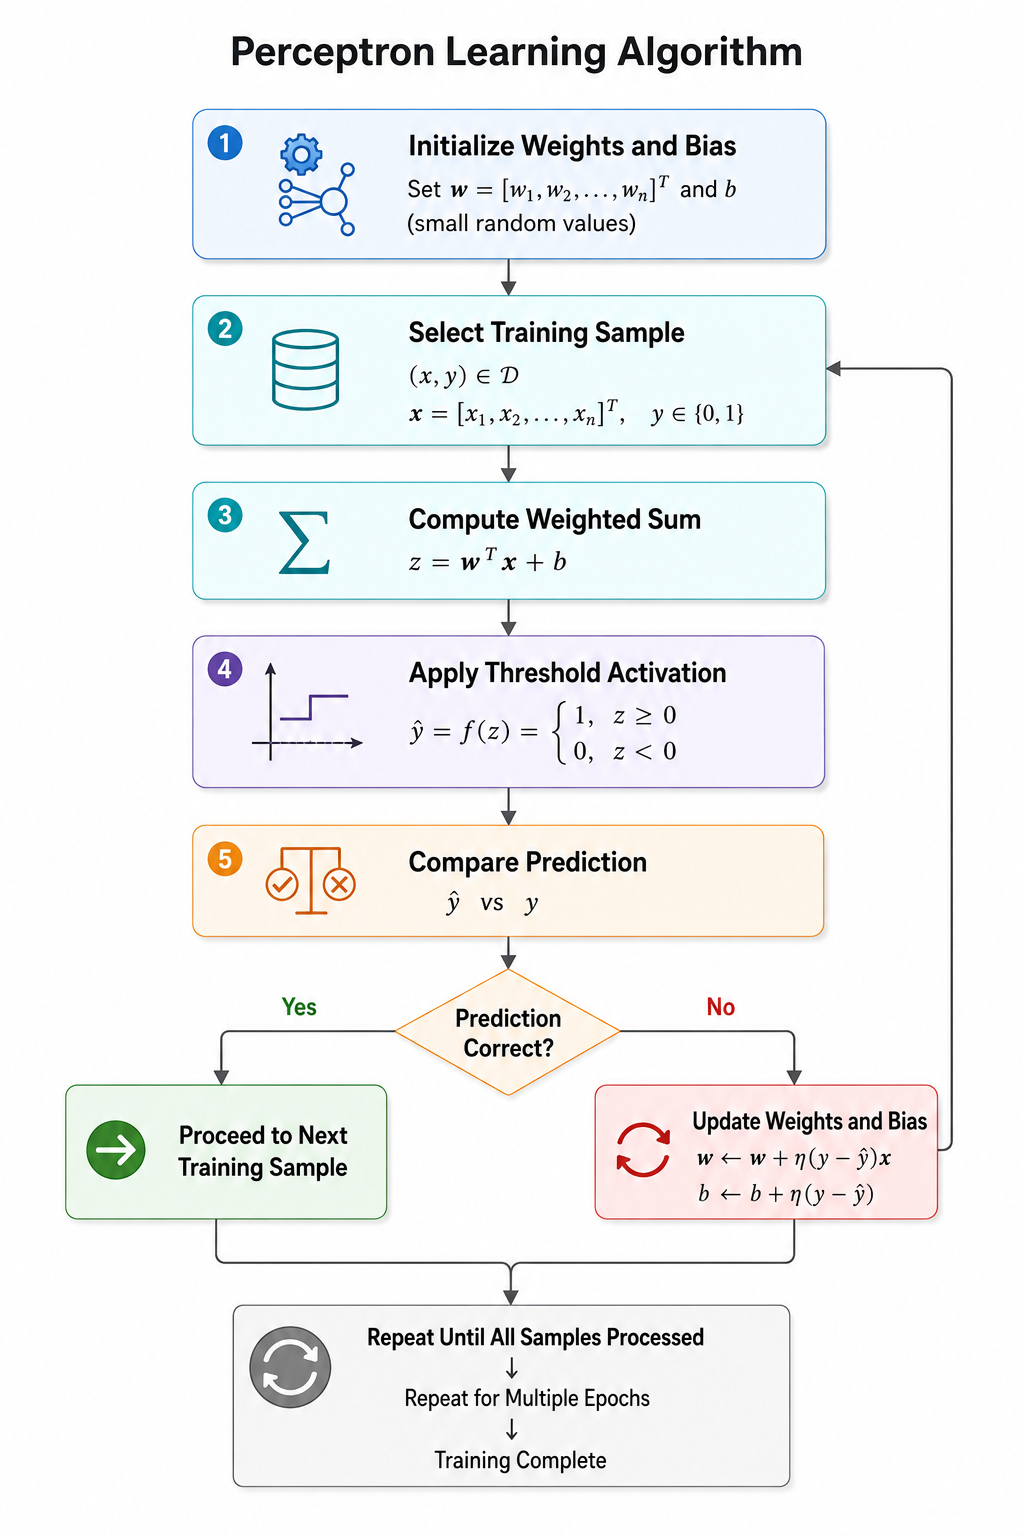
\includegraphics[width=0.95\textwidth]{figures/1-3 figure.png}
\end{figure}
\clearpage

An important property of the Perceptron Learning Algorithm is described by the \textbf{Perceptron Convergence Theorem}, which states that if the training data are linearly separable, the algorithm is guaranteed to find a decision boundary after a finite number of updates. However, when the data are not linearly separable, the algorithm cannot converge to a perfect solution. This limitation motivates the study of one of the most famous problems in the history of neural networks: the XOR problem.

\section{The XOR Problem}

Although the Perceptron was a significant breakthrough in the development of artificial neural networks, it has an important limitation: it can correctly classify only \textbf{linearly separable} data. A dataset is said to be linearly separable if its classes can be separated by a single straight line (or, more generally, by a hyperplane).

One of the simplest examples of a non-linearly separable problem is the \textbf{Exclusive OR (XOR)} logical function. The XOR function produces an output of 1 only when its two inputs are different, as shown in Table~\ref{tab:xor}.

\begin{table}[h]
\centering
\caption{Truth table of the XOR function.}
\label{tab:xor}
\begin{tabular}{ccc}
\hline
$x_1$ & $x_2$ & XOR \\
\hline
0 & 0 & 0 \\
0 & 1 & 1 \\
1 & 0 & 1 \\
1 & 1 & 0 \\
\hline
\end{tabular}
\end{table}
\begin{figure}[h]
    \centering
    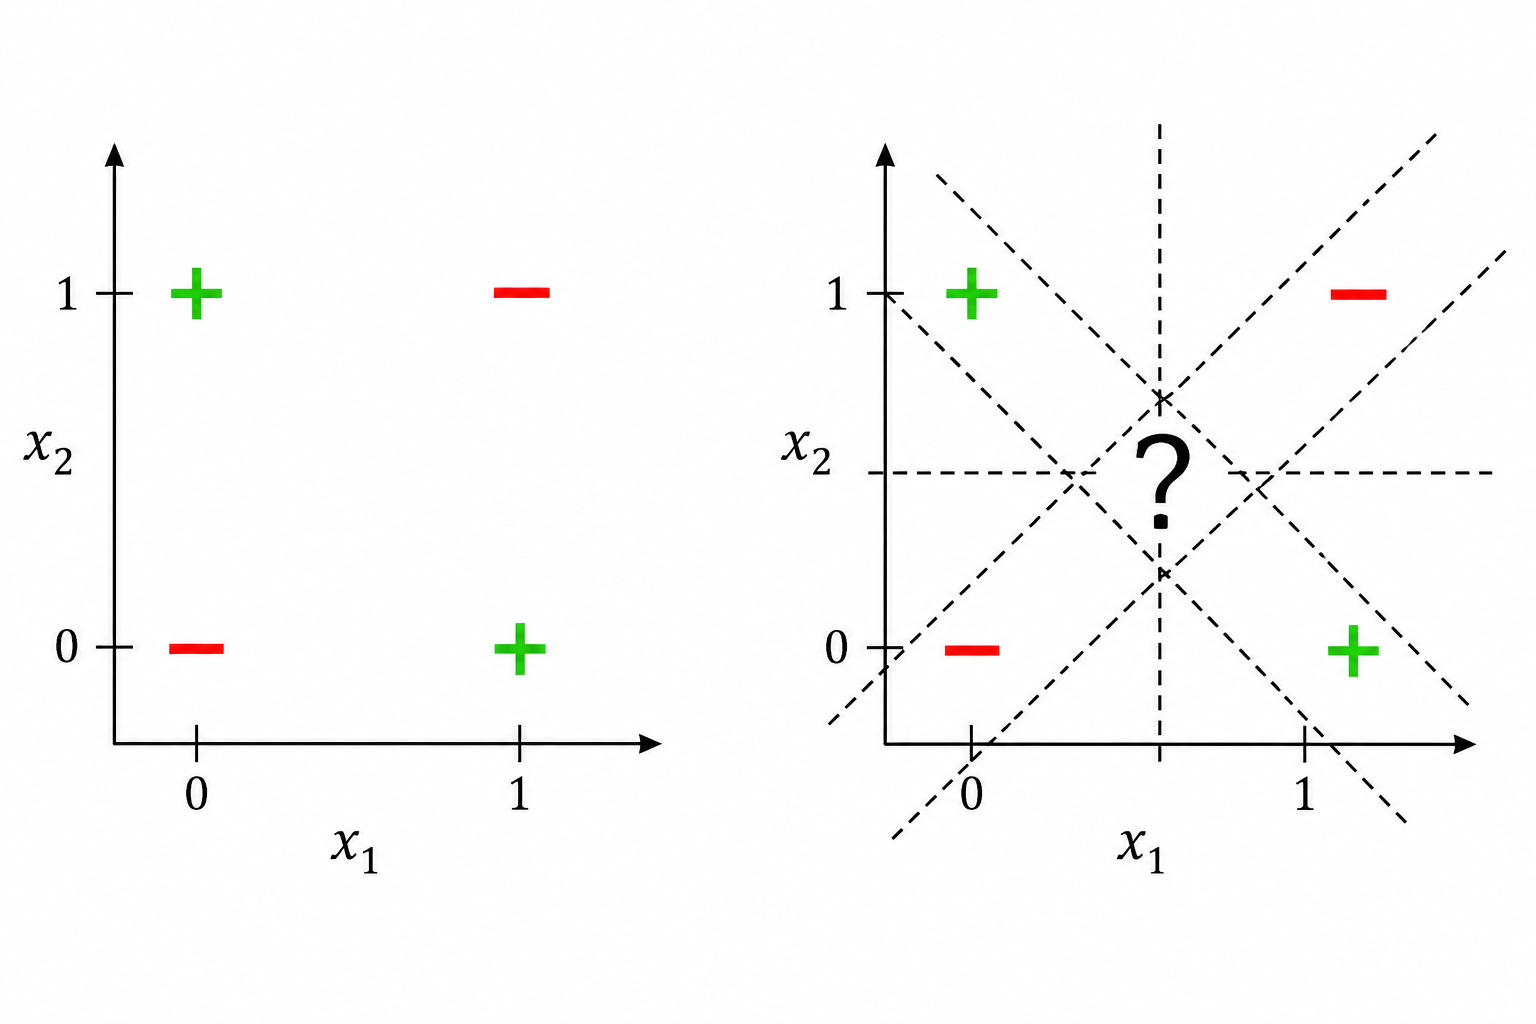
\includegraphics[width=0.95\textwidth]{figures/1-4.png}
\end{figure}

When these four input combinations are represented in a two-dimensional plane, no single straight line can separate the two classes. Since the Perceptron always learns a linear decision boundary, it is mathematically impossible for a single-layer Perceptron to solve the XOR problem.

This limitation was highlighted by Marvin Minsky and Seymour Papert in their influential 1969 book \textit{Perceptrons}. Their work demonstrated that single-layer neural networks are unable to represent certain simple functions, including XOR. As a result, research on neural networks declined for several years, a period that is often referred to as the \textbf{AI Winter}.

The XOR problem also revealed an important insight: some problems require models capable of learning \textbf{non-linear decision boundaries}. This challenge was eventually overcome by introducing one or more hidden layers between the input and output layers, giving rise to the \textbf{Multi-Layer Perceptron (MLP)}.

\section{Multi-Layer Perceptron (MLP)}

The limitations of the single-layer Perceptron motivated the development of more powerful neural network architectures capable of learning complex, non-linear relationships. The simplest extension is the \textbf{Multi-Layer Perceptron (MLP)}, which introduces one or more hidden layers between the input and output layers.

An MLP is a feedforward neural network composed of multiple layers of interconnected neurons. Information flows sequentially from the input layer through one or more hidden layers until it reaches the output layer. Each neuron performs the same basic computation introduced in the previous sections, while the hidden layers progressively transform the input into increasingly meaningful representations.

The addition of hidden layers greatly increases the expressive power of the network. Unlike a single-layer Perceptron, which can learn only linear decision boundaries, an MLP is capable of modeling highly complex and non-linear functions. This enables it to solve problems such as the XOR classification task and forms the basis of many modern deep learning models.

Figure~\ref{fig:mlp_architecture} illustrates the general architecture of a Multi-Layer Perceptron. The input layer receives the features from the dataset and passes them to the first hidden layer. Each hidden neuron computes a weighted sum of its inputs, adds a bias term, and produces an output that is forwarded to the next layer. This process continues through all hidden layers until the output layer generates the network's final prediction.

\begin{figure}[h]
    \centering
    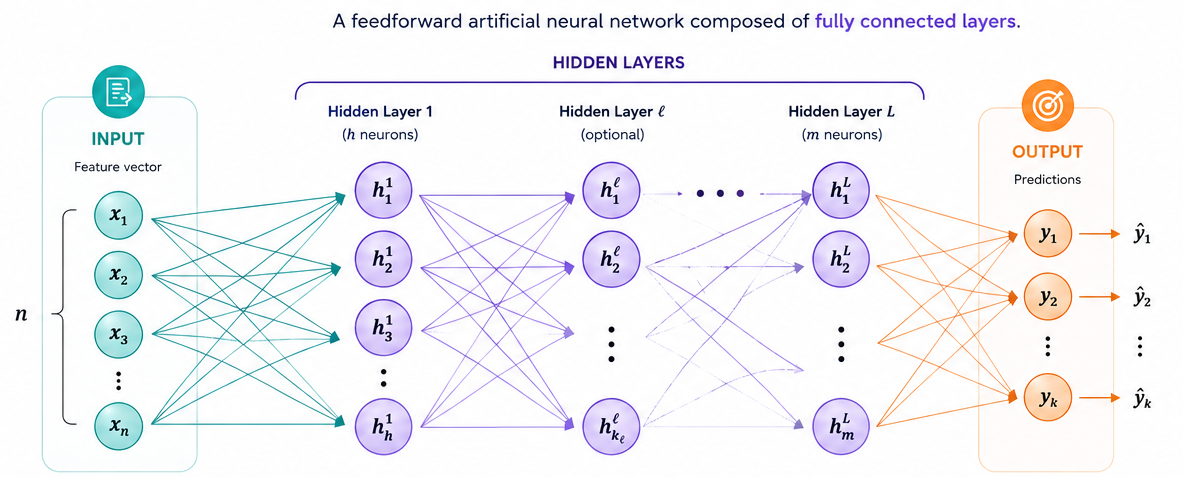
\includegraphics[width=0.95\textwidth]{figures/1-5.png}
    \caption{Architecture of a Multi-Layer Perceptron (MLP).}
    \label{fig:mlp_architecture}
\end{figure}
Although the architecture of an MLP is conceptually simple, stacking multiple layers alone is not sufficient to increase the network's learning capability. If every neuron performed only a linear transformation, the entire network would still behave as a single linear model, regardless of the number of hidden layers. To overcome this limitation, each neuron applies an \textbf{activation function}, introducing the non-linearity that enables deep neural networks to learn complex patterns.


\section{Activation Functions}

Without activation functions, a deep neural network is equivalent to a single layer.

Activation functions introduce non-linearity, allowing the network to approximate complex functions.

An ideal activation function should:
\begin{itemize}
    \item Introduce non-linearity (curved and complex decision boundaries, not just a straight line)
    \item Be differentiable (or almost everywhere differentiable)
    \item Be computationally efficient
    \item Avoid vanishing gradient
    \item Avoid exploding gradient
    \item Have a stable output range
\end{itemize}

\subsection{Sigmoid}

\begin{equation}
\sigma(x) = \frac{1}{1 + e^{-x}} \qquad \text{Range: } (0, 1)
\end{equation}

\sigmoidplot

Output values that resemble probabilities (e.g., $0.98 \to \text{very likely}$, $0.5 \to \text{uncertain}$, $0.02 \to \text{very unlikely}$).

\begin{advbox}[Sigmoid Summary]
\textbf{Advantages:}
\begin{itemize}
    \item Smooth and differentiable.
    \item Output interpretable as a probability.
    \item Works well for binary classification outputs.
\end{itemize}

\tcbline

\textbf{Disadvantages:}
\begin{itemize}
    \item \textbf{Vanishing Gradient:} For very large positive or negative inputs, $\sigma'(x) \approx 0$. The gradient becomes extremely small, slowing or stopping learning in deep networks.
    \item \textbf{Saturation:}
    \begin{equation}
    \text{For } x \gg 0, \quad \sigma(x) \approx 1; \qquad \text{For } x \ll 0, \quad \sigma(x) \approx 0
    \end{equation}
    Small changes in input barely affect the output.
    \item \textbf{Not Zero-Centered:} Outputs are always positive, which can lead to less efficient optimization because gradients tend to have the same sign.
\end{itemize}
\end{advbox}

\paragraph{Usage:}
\begin{itemize}
    \item \textbf{Hidden Layer:} Rarely used.
    \item \textbf{Output Layer:} Binary classification.
\end{itemize}

\subsection{Tanh (Hyperbolic Tangent)}

\begin{equation}
\tanh(x) = \frac{e^x - e^{-x}}{e^x + e^{-x}} \qquad \text{Range: } (-1, 1)
\end{equation}

\begin{equation}
\text{Derivative: } 1 - \tanh^2(x)
\end{equation}

\tanhplot

\begin{advbox}[Tanh Summary]
\textbf{Advantages:}
\begin{itemize}
    \item \textbf{Zero-Centered:} Output can be positive or negative. This generally leads to faster convergence than Sigmoid.
    \item \textbf{Larger Gradient Near Zero:} Learning is often faster around the origin.
\end{itemize}

\tcbline

\textbf{Disadvantages:}
\begin{itemize}
    \item \textbf{Vanishing Gradients.}
    \item \textbf{Saturation for large positive and negative $x$:}
    \begin{align*}
        10 &\rightsquigarrow 1 & 50 &\rightsquigarrow 1 \\
        100 &\rightsquigarrow 1 & 1000 &\rightsquigarrow 1 \\
        10 \times 10^{50} &\rightsquigarrow 1 & -10 \times 10^{50} &\rightsquigarrow -1
    \end{align*}
\end{itemize}
\end{advbox}

\paragraph{Usage:} Common in RNNs; less common in modern feed-forward networks.

\subsection{ReLU (Rectified Linear Unit)}

\begin{equation}
f(x) = \max(0, x) \qquad \text{Range: } [0, +\infty)
\end{equation}

\begin{equation}
\text{Derivative: } f'(x) = \begin{cases} 1 & x > 0 \\ 0 & x < 0 \end{cases}
\end{equation}
\reluplot
\textit{Note: At $x = 0$, $f'(0)$ is non-differentiable. Most Python frameworks define it as 0 or 1.}

\begin{advbox}[ReLU Summary]
\textbf{Advantages:}
\begin{itemize}
    \item \textbf{Extremely Fast:} Only requires a comparison with zero.
    \item \textbf{Sparse Activation:} Negative inputs become exactly zero, making many neurons inactive (improves efficiency and sometimes reduces overfitting).
    \item \textbf{Reduces Vanishing Gradient:} For positive inputs, $f'(x) = 1$. The gradient passes through unchanged.
\end{itemize}

\tcbline

\textbf{Disadvantages:}
\begin{itemize}
    \item \textbf{Dying ReLU:} If a neuron's output becomes permanently negative ($f(x) = 0$), its gradient is also zero, so the neuron may never recover.
    \item \textbf{Unbounded Output:} Large activations can sometimes contribute to exploding activation if not managed properly.
\end{itemize}
\end{advbox}

\paragraph{Usage:} The default choice for hidden layers in many neural networks, including CNNs and MLPs.

\subsection{Leaky ReLU \& Parametric ReLU (PReLU)}

\begin{equation}
f(x) = \begin{cases} x & x > 0 \\ \alpha x & x < 0 \end{cases}, \qquad \alpha = 0.01 \qquad \text{Range: } (-\infty, +\infty)
\end{equation}

\begin{equation}
f'(x) = \begin{cases} 1 & x > 0 \\ \alpha & x < 0 \end{cases}
\end{equation}

\leakyreluplot

Invented to solve the Dying ReLU problem by allowing a small, non-zero gradient when the input is negative.

\begin{advbox}[Leaky ReLU Summary]
\textbf{Advantages:}
\begin{itemize}
    \item Reduces the chance of dead neurons.
    \item Still computationally efficient.
    \item Preserves gradient flow for negative inputs.
\end{itemize}

\tcbline

\textbf{Disadvantages:}
\begin{itemize}
    \item Introduces a hyperparameter ($\alpha$).
    \item Usually offers only modest improvements over ReLU.
\end{itemize}
\end{advbox}

\paragraph{Usage:} Used when standard ReLU leads to many dead neurons.

\paragraph{Parametric ReLU (PReLU):} Instead of fixing $\alpha$, the network learns it during training ($\alpha$ is a trainable parameter).
\begin{itemize}
    \item \textbf{Range:} $(-\infty, +\infty)$
    \item \textbf{Usage:} Sometimes used in computer vision models.
\end{itemize}

\subsection{ELU (Exponential Linear Unit)}

\begin{equation}
f(x) = \begin{cases} x & x > 0 \\ \alpha(e^x - 1) & x \le 0 \end{cases} \qquad \text{Range: } (-\infty, +\infty)
\end{equation}

\eluplot

\begin{advbox}[ELU Summary]
\textbf{Advantages:}
\begin{itemize}
    \item Smooth transition near zero.
    \item Negative outputs are allowed, making activations closer to zero-centered.
    \item Can converge faster than ReLU in some settings.
\end{itemize}

\tcbline

\textbf{Disadvantages:}
\begin{itemize}
    \item More computationally expensive because it uses the exponential function.
    \item Still has a saturation region for very negative inputs.
\end{itemize}
\end{advbox}

\paragraph{Usage:} Sometimes used instead of ReLU, though less common today.

\subsection{GELU (Gaussian Error Linear Unit)}

\begin{equation}
\text{GELU}(x) = x \Phi(x) \qquad \text{Range: } (-\infty, +\infty)
\end{equation}
where $\Phi(x)$ is the Cumulative Distribution Function (CDF) of the standard normal distribution.

A common approximation is:
\begin{equation}
\text{GELU}(x) \approx 0.5x \left( 1 + \tanh\left( \sqrt{\frac{2}{\pi}} \left( x + 0.044715 x^3 \right) \right) \right)
\end{equation}

\geluplot

Unlike ReLU, which either keeps or discards an input, GELU smoothly scales the input based on its magnitude.

\begin{advbox}[GELU Summary]
\textbf{Advantages:}
\begin{itemize}
    \item Smooth and differentiable.
    \item Excellent empirical performance in Transformers.
    \item Often leads to better accuracy than ReLU in language models.
\end{itemize}

\tcbline

\textbf{Disadvantages:}
\begin{itemize}
    \item Computationally more expensive than ReLU.
    \item Harder to compute analytically.
\end{itemize}
\end{advbox}

\paragraph{Usage:} Widely used in Transformer architectures, including models like BERT and GPT.

\subsection{Softmax}

For outputs $z_1, z_2, \dots, z_K$:
\begin{equation}
\text{Softmax}(z_i) = \frac{e^{z_i}}{\sum_{j=1}^{K} e^{z_j}}
\end{equation}

\softmaxplot

\begin{propertybox}[Softmax Properties]
\begin{itemize}
    \item Every output is between 0 and 1, and $\sum_{i=1}^K \text{Softmax}(z_i) = 1$.
    \item Produces a probability distribution over classes.
\end{itemize}
\end{propertybox}

\begin{advbox}[Softmax Summary]
\textbf{Advantages:}
\begin{itemize}
    \item Ideal for multi-class classification.
    \item Easy to interpret probabilistically.
\end{itemize}

\tcbline

\textbf{Disadvantages:}
\begin{itemize}
    \item Computationally expensive for very large numbers of classes.
    \item Can become numerically unstable if implemented naively.
\end{itemize}
\end{advbox}

\paragraph{Usage:} Always in the output layer for multi-class classification.

\subsection{Activation Selection Summary}

\begin{table}[h!]
\centering
\caption{Common Activation Functions by Network Type}
\begin{tabular}{ll}
\toprule
\textbf{Architecture / Task} & \textbf{Common Activation Function} \\
\midrule
MLP or CNN & ReLU or Leaky ReLU (if dead neurons occur) \\
Transformer Models & GELU, SwiGLU, or SiLU \\
Binary Classification & Sigmoid \\
Multi-Class Classification & Softmax (or logits with cross-entropy loss) \\
RNN & Tanh \\
\bottomrule
\end{tabular}
\end{table}

\clearpage

\section{Forward Propagation, Backpropagation \& Training Dynamics}

\subsection{Forward Propagation}

Moving information from input toward output: $x \rightsquigarrow \hat{y}$.

Forward propagation is the process by which a Multi-Layer Perceptron (MLP) transforms an input vector into a prediction by passing information sequentially from the input layer to the output layer. Given an input vector $x$, each neuron in the first hidden layer computes a weighted sum of its inputs followed by the addition of a bias term:
\begin{equation}
z^{(1)} = W^{(1)} x + b^{(1)}
\end{equation}

After that, we pass it into an activation function to produce (non-linear) hidden layer activations:
\begin{equation}
a^{(1)} = f\left(z^{(1)}\right)
\end{equation}

The activation function introduces non-linearity into the network, enabling it to learn complex relationships between the input feature and the target output. The output of one layer becomes the input to the next layer, and this process is repeated for every hidden layer $l$:
\begin{align}
z^{(l)} &= W^{(l)} a^{(l-1)} + b^{(l)} \\
a^{(l)} &= f\left(z^{(l)}\right)
\end{align}

After propagating through all hidden layers, we apply the output activation function to generate the network's prediction $\hat{y}$:
\begin{equation}
\hat{y} = g\left(z^{(L)}\right)
\end{equation}
where $g(\cdot)$ depends on the learning task:
\begin{itemize}
    \item \textbf{For binary classification:} Sigmoid function
    \item \textbf{For multi-class classification:} Softmax
    \item \textbf{For regression problems:} Any linear function
\end{itemize}

After we get $\hat{y}$ (prediction), it is compared with the true target $y$ using a loss function such as:
\begin{itemize}
    \item \textbf{MSE} (for regression)
    \item \textbf{Cross-Entropy Loss} (for categorical):
    \begin{equation}
    L = -\sum_{i} y_i \log(p_i)
    \end{equation}
    where $y_i$ is the one-hot encoded true label and $p_i$ is the probability from Softmax.
\end{itemize}
It measures how different the predicted probabilities are from the true labels.

\subsection{Backward Propagation}

Used to optimize the parameters of a Multilayer Perceptron (MLP) by minimizing the prediction error. After forward propagation, the network evaluates the discrepancy between $\hat{y}$ and $y$ using a loss function (MSE or Cross-Entropy). The objective of backward propagation is to determine how much each weight and bias contributed to this error and to compute the gradients required for updating the network parameters. This is accomplished using the \textbf{Chain Rule} of differential calculus, which allows the gradient of the loss function to be propagated backward from the output layer to the input layer.

\paragraph{Chain Rule:} If a function is composed of several nested functions $L = f(g(h(x)))$, the derivative of $L$ with respect to $x$ is obtained by multiplying each intermediate derivative:
\begin{equation}
\frac{\partial L}{\partial x} = \frac{\partial L}{\partial f} \cdot \frac{\partial f}{\partial g} \cdot \frac{\partial g}{\partial h} \cdot \frac{\partial h}{\partial x}
\end{equation}

To illustrate this concept, consider a single neuron with:
\begin{align}
z &= w x + b \\
a &= f(z) \\
\text{Loss: } L &= L(a)
\end{align}

\begin{equation}
\frac{\partial L}{\partial w} = \frac{\partial L}{\partial a} \cdot \frac{\partial a}{\partial z} \cdot \frac{\partial z}{\partial w}
\end{equation}

After calculating the gradients for all layers, the network updates its parameters using an optimization algorithm such as Gradient Descent. The weights and biases are adjusted in the direction that minimizes the loss according to the update rules:
\begin{align}
w_{\text{new}}^{(l)} &= w_{\text{old}}^{(l)} - \eta \frac{\partial L}{\partial w^{(l)}} \\
b_{\text{new}}^{(l)} &= b_{\text{old}}^{(l)} - \eta \frac{\partial L}{\partial b^{(l)}}
\end{align}
where $\eta$ is the learning rate.

\subsection{Vanishing Gradient Problem}

The vanishing gradient problem is one of the most significant challenges encountered when training deep neural networks using the backpropagation algorithm. It occurs when the gradients of the loss function with respect to the network parameters become progressively smaller as they are propagated backward from the output layer to the earlier hidden layers. As a result, the weights of neurons located near the input layer receive extremely small updates, preventing them from learning meaningful features. Consequently, the training process becomes very slow or may even stop entirely, leading to poor model performance and difficulty in optimizing deep neural networks.

The origin of the vanishing gradient problem lies in the repeated application of the chain rule during backpropagation.

For example, suppose each derivative has an average value of $0.5$. For a network with 10 hidden layers, the gradient becomes:
\begin{equation}
0.5^{10} = 0.00097
\end{equation}
For 20 hidden layers:
\begin{equation}
0.5^{20} = 9.54 \times 10^{-7}
\end{equation}
which is practically zero. The weight updates computed using Gradient Descent:
\begin{equation}
w_{\text{new}} = w_{\text{old}} - \eta \frac{\partial L}{\partial w}
\end{equation}
become extremely small because $\frac{\partial L}{\partial w} \approx 0$. The weights remain unchanged during training, and the network fails to learn useful representations.

The vanishing gradient problem is particularly severe when using activation functions whose derivatives are bounded between $0$ and $1$, such as Sigmoid and Tanh.

ReLU has a derivative equal to $1$ for positive inputs, allowing gradients to propagate through many layers without rapidly shrinking. That is why ReLU has become the standard activation function for most deep neural networks.

\subsection{Exploding Gradient Problem}

The exploding gradient problem occurs during backpropagation when gradients become excessively large as they propagate from the output layer to the earlier layers. Unlike the vanishing gradient producing excessively small weight updates, exploding gradients increase exponentially, producing excessively large weight updates that destabilize training. This often causes the loss to oscillate, diverge, or produce numerical overflow ($\infty$ or NaN), preventing the network from converging.

The exploding gradient problem arises from the repeated application of the chain rule during backpropagation.

For example:
\begin{equation}
2^{10} = 1024 \quad \rightsquigarrow \quad 2^{20} = 1048576
\end{equation}

Large weight values can further amplify this effect during forward propagation.

\begin{examplebox}[Exploding Update Example]
Suppose $w = 0.8$, $\eta = 0.01$, and $\frac{\partial L}{\partial w} = 5000$. Then:
\begin{equation}
w_{\text{new}} = 0.8 - 0.01 \times 5000 = -49.2
\end{equation}
Instead of a small adjustment, the weight changes from $0.8$ to $-49.2$ in a single update. Such a drastic modification significantly alters network behavior, creating a cycle of numerical instability.
\end{examplebox}

\paragraph{Mitigation Techniques:}
\begin{itemize}
    \item \textbf{Gradient Clipping:} Limit the magnitude of the gradient before updating the parameters by setting a threshold $c$.
    \item \textbf{Proper Weight Initialization:} Such as Xavier (Glorot) initialization.
    \item \textbf{Adaptive Optimization Algorithms:} Such as Adam and RMSProp.
\end{itemize}

\subsection{Heuristics for Hidden Layer Neurons}

Best heuristics used to initialize the number of neurons in hidden layers:

Between the input and output sizes ($N_o < N_h < N_i$):
\begin{itemize}
    \item \textbf{Two-Thirds Rule:}
    \begin{equation}
    N_h = \frac{2}{3} N_i + N_o \qquad (\text{most common})
    \end{equation}
    \item \textbf{Average Rule:}
    \begin{equation}
    N_h = \frac{N_i + N_o}{2}
    \end{equation}
    \item \textbf{Start Small and Increase Gradually:} $N_h = \{16, 32, 64, 128, \dots\}$
    \item \textbf{Grid Search:} Test all combinations $\{32, 64, 128\}$ and learning rates $\{0.1, 0.01, 0.001\}$ across 3 hidden layers. This tests $3 \times 3 \times 3 = 27$ models, which is computationally expensive.
    \item \textbf{Random Search:} Try random combinations.
\end{itemize}

\subsection{Epoch and Batch Concepts}

\begin{description}
    \item[Epoch:] Complete pass through the entire training dataset. Calculate gradient, update weight, and repeat.
    \item[Batch (or mini-batch):] Number of training examples processed in one forward and backward pass.
\end{description}

\paragraph{Example:} If we have 1000 images and batch size = 100, the model looks at 100 images, calculates the error, and updates weights. It does this 10 times to see all the data (1 epoch).

\paragraph{Analogy:}
\begin{itemize}
    \item Reading the whole book once: \textbf{1 Epoch}
    \item 1 Chapter: \textbf{A Batch}
    \item 1 Page: \textbf{A Single Data Point}
\end{itemize}

\clearpage

\section{Optimizers \& Learning Rate Schedules}

Training a neural network means solving: find parameters $w$ that minimize Loss. The loss surface for a real network is high-dimensional, non-convex, full of saddle points, and noisy. The optimizer is the rule that decides how $w$ updates at each step, given the gradient.

Every optimizer answers three questions:
\begin{enumerate}
    \item Which direction do we step?
    \item How big is the step?
    \item Do we remember anything from previous steps?
\end{enumerate}

\subsection{Vanilla Gradient Descent (GD)}

\begin{equation}
\text{Update Rule: } w = w - \eta \frac{\partial L}{\partial w}
\end{equation}

\begin{enumerate}[label=\Roman*.]
    \item \textbf{Batch GD (BGD):} Gradient computed on the whole dataset. Accurate but slow, one update per epoch.
    \item \textbf{Stochastic GD (SGD):} Gradient computed on one sample. Fast, very noisy (high variance, unbiased).
    \item \textbf{Mini-Batch SGD:} Gradient on a batch of 32 / 64 / 256 samples. The standard in practice — balances noise and speed (low variance, unbiased).
\end{enumerate}

\paragraph{Problems with plain GD / SGD:}
\begin{itemize}
    \item \textbf{Oscillations:} Oscillates badly in narrow valleys (ravines). It zig-zags across the steep direction instead of moving smoothly along the shallow direction.
    \item \textbf{Saddle Points:} Gets stuck or slows drastically near saddle points (very common in high dimensions — more common than local minima).
    \item \textbf{Static Learning Rate:} Same learning rate for every parameter, even though some parameters may need bigger or smaller steps.
\end{itemize}

\subsection{Saddle Points}

In the high dimensional landscapes of Deep Learning, saddle points are significantly more problematic than local minima.

While intuition from 2D or 3D optimization suggests that reaching a point where $\frac{dL}{dw} = 0$ usually means you have found a local minimum, in reality, your model is far more likely to be stuck on a saddle point.

\begin{itemize}
    \item A \textbf{saddle point} is a critical point where the function reaches a plateau in at least one direction (the gradient is zero) but increases in some directions and decreases in others.
    \item \textbf{The Geometry:} Think of a mountain pass between two peaks. If you are standing in the middle, the slope is zero in the direction of the pass (you are at a ``minimum'' relative to the mountains) but you are at a ``maximum'' relative to the path going over the pass.
    \item \textbf{The Hessian Perspective:} The Hessian matrix $H = \frac{d^2 L}{d w^2}$ contains the curvature information:
    \begin{itemize}
        \item \textbf{Local minimum:} All eigenvalues of $H$ are positive (Positive definite).
        \item \textbf{Local maximum:} All eigenvalues of $H$ are negative (Negative definite).
        \item \textbf{Saddle Point:} The Hessian has both positive and negative eigenvalues (Indefinite).
    \end{itemize}
\end{itemize}

\begin{center}
\begin{tikzpicture}[scale=0.9, baseline]
  % 3D Loss Landscape Contour & Surface representation
  \fill[boxbg,rounded corners=4pt] (-6,-2.8) rectangle (6,3.5);
  
  % Contour ellipses at bottom
  \draw[borderblue!80, line width=0.4pt] (0,-1.8) ellipse (4.5cm and 0.7cm);
  \draw[borderblue!80, line width=0.4pt] (-2.2,-1.8) ellipse (1.2cm and 0.4cm);
  \draw[borderblue!80, line width=0.4pt] (2.2,-1.8) ellipse (1.2cm and 0.4cm);
  
  % Surface mesh outline
  \draw[bookcurve, color=secondaryblue] plot [smooth, tension=0.7] coordinates {(-4.5,0) (-2.5,2.2) (0,1.2) (2.5,2.2) (4.5,0)};
  \draw[bookcurve, color=primaryblue] plot [smooth, tension=0.7] coordinates {(-4.5,0) (-2.2,-1.5) (0,-0.4) (2.2,-1.5) (4.5,0)};
  
  % Saddle Point and Max/Min points
  \filldraw[accentred] (0,1.2) circle (2.5pt) node[above=4pt, font=\sffamily\bfseries\small, color=primaryblue] {Saddle Point};
  \filldraw[primaryblue] (-2.5,2.2) circle (2pt) node[above=2pt, font=\sffamily\scriptsize] {Local Maximum};
  \filldraw[primaryblue] (2.5,2.2) circle (2pt) node[above=2pt, font=\sffamily\scriptsize] {Local Maximum};
  \filldraw[secondaryblue] (-2.2,-1.5) circle (2pt) node[below=2pt, font=\sffamily\scriptsize] {Local Minimum};
  \filldraw[secondaryblue] (2.2,-1.5) circle (2pt) node[below=2pt, font=\sffamily\scriptsize] {Local Minimum};

  % Projection lines
  \draw[dashed, warmgray!70] (0,1.2) -- (0,-0.4);
  \draw[dashed, warmgray!70] (-2.2,-1.5) -- (-2.2,-1.8);
  \draw[dashed, warmgray!70] (2.2,-1.5) -- (2.2,-1.8);
\end{tikzpicture}
\end{center}

\begin{itemize}
    \item To identify if you are at a saddle point versus a local minimum, you look at the spectrum of the Hessian. If the gradient is near zero, we use eigen-decomposition of the Hessian.
    \item If we find any negative eigenvalues, you are at a saddle point.
    \item The eigenvector corresponding to the most negative eigenvalue points in the direction of the steepest descent to escape the saddle point.
\end{itemize}

\subsection{Momentum}

Keep a velocity that accumulates past gradients:
\begin{align}
v_t &= \beta v_{t-1} + (1 - \beta) \frac{\partial L}{\partial w} \\
w_t &= w_{t-1} - \eta v_t
\end{align}
$\beta$ is typically $0.9$ (meaning velocity is 90\% memory, 10\% new gradient).

\begin{examplebox}[Momentum Calculation]
Given $\beta = 0.9$, $\eta = 0.1$, and $\frac{\partial L}{\partial w} = 2$:
\begin{align*}
v_1 &= 0.9 \times 0 + 0.1 \times 2 = 0.2, \quad &w_1 &= w_0 - 0.1 \times 0.2 = -0.02 \\
v_2 &= 0.9 \times 0.2 + 0.1 \times 2 = 0.38, \quad &w_2 &= w_1 - 0.1 \times 0.38 = -0.058
\end{align*}
\end{examplebox}

Notice: $v$ keeps growing when gradient keeps pointing the same way. This is what accelerates convergence along consistent directions, and cancels out in oscillating directions (because opposite-sign gradients average out).

\subsection{Nesterov Accelerated Gradient (NAG)}

A smarter variant; you compute the gradient not at the current $w$, but at the look-ahead position resulting from current velocity (at the position reached after applying current velocity). This corrects overshooting slightly earlier than classical momentum.

\begin{align}
w_{\text{lookahead}} &= w_{t-1} - \eta \beta v_{t-1} \\
v_t &= \beta v_{t-1} + (1 - \beta) \frac{\partial L}{\partial w_{\text{lookahead}}} \\
w_t &= w_{t-1} - \eta v_t
\end{align}

So NAG is a ``look-ahead'' version of momentum; it calculates the gradient at the predicted next position ($w_{t-1} - \eta \beta v_{t-1}$) rather than the current position, allowing for more responsive corrections.

\subsection{Adaptive Learning Rate Methods}

The core idea: give each parameter its own effective learning rate, based on how large its past gradients have been.

\subsubsection{Adagrad}

Accumulate the sum of squared gradients per parameter:
\begin{align}
G_t &= G_{t-1} + \left( \frac{\partial L}{\partial w} \right)^2 \\
w_t &= w_{t-1} - \frac{\eta}{\sqrt{G_t} + \varepsilon} \frac{\partial L}{\partial w}
\end{align}

\begin{itemize}
    \item Parameters that get large/frequent gradients $\to G$ grows $\to$ step shrinks.
    \item Parameters that get small/rare gradients $\to$ step stays large.
\end{itemize}

Adagrad adapts the learning rate based on the sum of squares of historical gradients. It performs well on sparse data (like word embeddings), but suffers from a vanishing learning rate because the denominator grows monotonically.

\subsubsection{RMSProp}

Solves Adagrad's decay issue by using an exponentially weighted moving average of squared gradients, allowing it to forget older, less relevant gradients:
\begin{align}
S_t &= \beta S_{t-1} + (1 - \beta) \left( \frac{\partial L}{\partial w} \right)^2 \\
w_t &= w_{t-1} - \frac{\eta}{\sqrt{S_t} + \varepsilon} \frac{\partial L}{\partial w}
\end{align}

Now old gradients fade out instead of accumulating forever, so the learning rate doesn't die. $\beta$ is typically $0.99$ or $0.999$.

\subsubsection{Adam (Adaptive Moment Estimation)}

Combines both Momentum (first moment) and RMSProp (second moment):
\begin{align}
m_t &= \beta_1 m_{t-1} + (1 - \beta_1) \frac{\partial L}{\partial w} \qquad (\text{mean of gradients}) \\
v_t &= \beta_2 v_{t-1} + (1 - \beta_2) \left( \frac{\partial L}{\partial w} \right)^2 \qquad (\text{second moment}) \\
\hat{m}_t &= \frac{m_t}{1 - \beta_1^t} \qquad (\text{bias correction}) \\
\hat{v}_t &= \frac{v_t}{1 - \beta_2^t} \qquad (\text{bias correction}) \\
w_t &= w_{t-1} - \frac{\eta \hat{m}_t}{\sqrt{\hat{v}_t} + \varepsilon}
\end{align}
\textbf{Default parameters:} $\beta_1 = 0.9$, $\beta_2 = 0.999$, $\varepsilon = 10^{-8}$.

\paragraph{Why bias correction?} $m$ and $v$ start at $0$, so early in training they are biased toward $0$. Dividing by $1 - \beta_1^t$ for $m_t$ and $1 - \beta_2^t$ for $v_t$ compensates. At $t=1$, with $\beta_2 = 0.999$, $1 - \beta_2^1 = 0.001$, so $\hat{v}_1 = v_1 / 0.001$---a large correction that shrinks as $t$ grows and the bias fades naturally.

Adam is the default choice for most deep learning today because it is robust to learning rate choice and works well out of the box on noisy, sparse, non-stationary problems.

\subsubsection{AdamW (Decoupled Weight Decay)}

Standard Adam applies weight decay ($L_2$ regularization) by adding $\lambda w$ to the gradient before the Adam math. But this means weight decay gets scaled by the adaptive learning rate too, which is not what you want (regularization strength shouldn't depend on gradient history).

AdamW decouples it:
\begin{equation}
w_t = w_{t-1} - \eta \left( \frac{\hat{m}_t}{\sqrt{\hat{v}_t} + \varepsilon} \right) - \eta \lambda w_{t-1}
\end{equation}

AdamW fixed this by applying weight decay directly to the weight (post update), ensuring that every weight is penalized proportionally to its magnitude, regardless of its historical gradient. This leads to significantly better generalization in deep neural networks and Transformers.

This is now the standard optimizer for training Transformers, LLMs, and most modern vision models (ViT, ResNet, etc.).

\subsection{Optimizer vs Schedule}

\begin{itemize}
    \item \textbf{Optimizer (e.g., AdamW):} Responsible for the weight update equations at each time step $t$. It decides how to move based on the gradient and momentum.
    \item \textbf{Schedule (Learning Rate Schedule):} Determines the magnitude of the step size (learning rate) that the optimizer takes at each step.
    \item \textbf{Interaction:} AdamW calculates velocity and gradient, while the scheduler controls step size. Without a scheduler, AdamW would take very large steps in the beginning because velocity is uncalibrated ($\hat{v} \approx 0$), leading to unstable gradient exploration.
\end{itemize}

\paragraph{Learning Rate Schedules:}
\begin{itemize}
    \item \textbf{Step Decay:} Reducing the learning rate by a factor (e.g., $\times 0.1$) every fixed number of epochs.
    \item \textbf{Cosine Annealing:} Making the learning rate follow a cosine curve to gradually decrease to near zero by the end of training (the most common).
    \item \textbf{Warmup:} Starting with a very small learning rate and increasing it gradually over initial steps. This is essential in Transformers because velocity is unstable in the beginning, and starting with a large learning rate can cause model collapse.
    \item \textbf{One-Cycle Policy:} Increasing the learning rate then decreasing it during training, while moving velocity inversely (high velocity when learning rate is low and vice versa).
\end{itemize}

\subsection{First-Order vs Second-Order Geometry}

\begin{itemize}
    \item \textbf{First-Order Methods (e.g., AdamW):} First-order methods use only the first derivative (gradient) to estimate the direction of the minimum.
    \item \textbf{Second-Order Methods (e.g., Shampoo, Newton, K-FAC):} Advanced optimizers using second-order methods do not stop at looking at gradient direction, but calculate curvature using second derivatives.
\end{itemize}

\subsection{Advanced Methods}

Methods attempting to understand loss function curvature for faster convergence, though computationally expensive:
\begin{itemize}
    \item \textbf{Newton's Method:} Uses the Hessian Matrix containing second derivatives of the loss function. Its complexity is $O(n^3)$, making it computationally infeasible for large models.
    \item \textbf{Natural Gradient Descent:} Uses the Fisher Information Matrix; more accurate but still expensive.
    \item \textbf{K-FAC:} Uses Kronecker-factored approximate curvature on second derivatives, enabling practical application in deep neural networks.
    \item \textbf{Shampoo:} Recent optimizer from Google. Acts as a second-order method by treating each layer independently to accelerate convergence.
    \item \textbf{LAMB:} Designed specifically for training large models with massive batch sizes by adapting the learning rate layer-wise.
    \item \textbf{Lion, Sophia, Adan (2023--2024 Optimizers):} Modern optimizers aimed at making LLM training more memory- and time-efficient using clever estimates of derivatives (e.g., diagonal Hessian in Sophia, sign operation in Lion).
\end{itemize}

\paragraph{Advanced Methods Summary (Shampoo / Second-Order):} Future research directions attempting to find shortcut paths by understanding landscape curvature (Hessian) instead of relying solely on the refined gradient estimates that AdamW uses.
